
\documentclass{standalone}
\usepackage{tikz}
\usetikzlibrary{intersections,shapes.arrows}

\newcommand\Dist[1]{\phantom{\rule{#1}{4pt}}}

\begin{document}

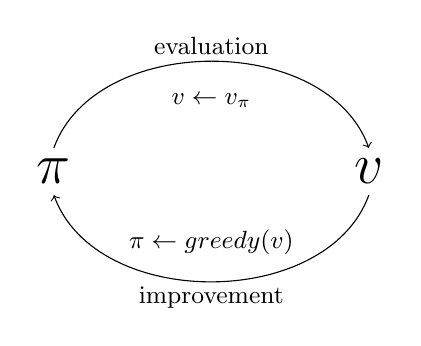
\begin{tikzpicture}

\node at (0,0) (pi) {\huge $\pi$};
\node at (4,0) (pi) {\huge $v$};

\draw[->] (0,0.3) to[out=70, in=110] (4,0.3);

\draw[->] (4,-0.3)to[out=-110, in=-70] (0,-0.3);

\node at (2,1.6) {\small evaluation};
\node at (2,-1.6) {\small improvement};
\node at (2,-0.9) {\small $\pi \leftarrow greedy(v)$};
\node at (2,0.9) {\small $v \leftarrow v_\pi$};
	
\end{tikzpicture}

\end{document}

